\documentclass[12pt,a4paper]{article}
\usepackage[utf8]{inputenc}
\usepackage[T1]{fontenc}
\usepackage{amsmath,amssymb,amsfonts}
\usepackage{graphicx}
\usepackage{booktabs}
\usepackage{geometry}
\usepackage{hyperref}
\usepackage{float}
\usepackage{caption}
\usepackage{subcaption}
\usepackage{enumitem}
\usepackage{xcolor}
\usepackage{fancyhdr}
\usepackage{listings}
\usepackage{multirow}
\usepackage{array}

\geometry{left=2.5cm,right=2.5cm,top=2.5cm,bottom=2.5cm}

\hypersetup{
    colorlinks=true,
    linkcolor=blue,
    filecolor=magenta,
    urlcolor=cyan,
    pdftitle={Three-Layer MLP for EuroSAT Classification},
}

\pagestyle{fancy}
\fancyhf{}
\fancyhead[L]{\small HW1: Three-Layer MLP Classifier}
\fancyhead[R]{\small \thepage}
\renewcommand{\headrulewidth}{0.4pt}

\lstset{
    basicstyle=\ttfamily\small,
    breaklines=true,
    frame=single,
    backgroundcolor=\color{gray!10},
    keywordstyle=\color{blue},
    commentstyle=\color{green!50!black},
    stringstyle=\color{red},
}

\title{\textbf{从零构建三层神经网络分类器\\实现EuroSAT地表覆盖图像分类}}
\author{实验报告}
\date{\today}

\begin{document}

\maketitle
\thispagestyle{empty}

\begin{abstract}
本实验从零实现了一个基于自动微分的三层多层感知机（MLP）分类器，在EuroSAT遥感图像数据集上进行训练，实现基于卫星图像的土地覆盖分类。整个系统不依赖PyTorch、TensorFlow等深度学习框架，仅使用NumPy进行矩阵运算，自主实现了计算图构建、反向传播自动微分、SGD优化器（含动量和L2正则化）、交叉熵损失函数以及学习率衰减策略。通过数据增强、模型容量扩展和超参数优化，最优模型在测试集上达到了74.42\%的分类准确率。报告详细介绍了模型结构、数据处理流程、训练过程可视化、第一层权重空间模式分析以及错例分析。
\end{abstract}

\tableofcontents
\newpage

%============================================================
\section{任务概述}
%============================================================

本实验要求手工搭建三层神经网络（MLP）分类器，在EuroSAT遥感图像数据集上进行训练，实现基于卫星图像的土地覆盖分类。核心要求包括：

\begin{enumerate}[leftmargin=2em]
    \item \textbf{自主实现自动微分与反向传播}：不使用PyTorch、TensorFlow等框架，仅使用NumPy进行矩阵运算；
    \item \textbf{模块化代码结构}：包含数据加载、模型定义、训练循环、测试评估、超参数查找五个模块；
    \item \textbf{模型与优化细节}：支持自定义隐藏层大小、多种激活函数切换、SGD优化器、学习率衰减、交叉熵损失和L2正则化；
    \item \textbf{超参数搜索}：利用网格搜索调节学习率、隐藏层大小、正则化强度等超参数；
    \item \textbf{测试评估}：输出分类准确率和混淆矩阵。
\end{enumerate}

%============================================================
\section{数据集介绍}
%============================================================

\subsection{EuroSAT数据集}

EuroSAT是一个用于地表覆盖分类的遥感图像基准数据集，基于Sentinel-2卫星采集的多光谱图像构建。本实验使用其RGB版本（EuroSAT\_RGB），包含10个类别，共27,000张64$\times$64像素的RGB彩色图像。各类别名称及样本数量如表~\ref{tab:dataset}所示。

\begin{table}[H]
\centering
\caption{EuroSAT\_RGB数据集各类别样本数量}
\label{tab:dataset}
\begin{tabular}{clcc}
\toprule
\textbf{类别编号} & \textbf{类别名称} & \textbf{中文名称} & \textbf{样本数量} \\
\midrule
0 & AnnualCrop & 一年生作物 & 3,000 \\
1 & Forest & 森林 & 3,000 \\
2 & HerbaceousVegetation & 草本植被 & 3,000 \\
3 & Highway & 高速公路 & 2,500 \\
4 & Industrial & 工业区 & 2,500 \\
5 & Pasture & 牧场 & 2,000 \\
6 & PermanentCrop & 多年生作物 & 2,500 \\
7 & Residential & 住宅区 & 3,000 \\
8 & River & 河流 & 2,500 \\
9 & SeaLake & 海洋/湖泊 & 3,000 \\
\midrule
 & \textbf{总计} & & \textbf{27,000} \\
\bottomrule
\end{tabular}
\end{table}

\subsection{数据预处理}

数据预处理流程如下：

\begin{enumerate}[leftmargin=2em]
    \item \textbf{图像缩放}：将原始64$\times$64图像缩放至32$\times$32，减少输入维度（3072维），降低计算开销；
    \item \textbf{像素归一化}：将像素值从[0, 255]缩放至[0, 1]；
    \item \textbf{数据增强}：对训练集进行水平翻转和垂直翻转，将训练样本从18,900扩充至56,700；
    \item \textbf{标准化}：使用训练集的逐像素均值$\mu$和标准差$\sigma$进行Z-score标准化：
    \begin{equation}
        x_{\text{norm}} = \frac{x - \mu}{\sigma}
    \end{equation}
    其中$\sigma < 10^{-8}$的维度被设为1以避免除零；
    \item \textbf{展平}：将32$\times$32$\times$3的图像展平为3072维向量，作为MLP的输入；
    \item \textbf{数据划分}：按7:1.5:1.5的比例随机划分训练集（18,900）、验证集（4,050）和测试集（4,050），随机种子为42。
\end{enumerate}

%============================================================
\section{模型结构}
%============================================================

\subsection{三层MLP架构}

本实验采用三层全连接神经网络（MLP），其数学表达式为：

\begin{align}
    \mathbf{h}_1 &= \sigma(\mathbf{W}_1 \mathbf{x} + \mathbf{b}_1) \\
    \mathbf{h}_2 &= \sigma(\mathbf{W}_2 \mathbf{h}_1 + \mathbf{b}_2) \\
    \mathbf{o} &= \mathbf{W}_3 \mathbf{h}_2 + \mathbf{b}_3
\end{align}

其中$\mathbf{x} \in \mathbb{R}^{3072}$为输入向量，$\mathbf{W}_1 \in \mathbb{R}^{3072 \times 1024}$、$\mathbf{W}_2 \in \mathbb{R}^{1024 \times 256}$、$\mathbf{W}_3 \in \mathbb{R}^{256 \times 10}$为权重矩阵，$\sigma$为激活函数，$\mathbf{o} \in \mathbb{R}^{10}$为输出logits。

最优模型的具体配置如表~\ref{tab:model_config}所示。

\begin{table}[H]
\centering
\caption{最优模型配置}
\label{tab:model_config}
\begin{tabular}{lc}
\toprule
\textbf{参数} & \textbf{值} \\
\midrule
输入维度 & 3072 (32$\times$32$\times$3) \\
隐藏层1大小 & 1024 \\
隐藏层2大小 & 256 \\
输出维度 & 10 \\
激活函数 & ReLU \\
权重初始化 & He初始化 ($\sqrt{2/n_{\text{in}}}$) \\
总参数量 & $\approx$3.4M \\
\bottomrule
\end{tabular}
\end{table}

\subsection{激活函数}

本实验支持三种激活函数，其定义及梯度如下：

\begin{itemize}[leftmargin=2em]
    \item \textbf{ReLU}：$f(x) = \max(0, x)$，$f'(x) = \mathbf{1}_{x>0}$
    \item \textbf{Sigmoid}：$f(x) = \frac{1}{1+e^{-x}}$，$f'(x) = f(x)(1-f(x))$
    \item \textbf{Tanh}：$f(x) = \tanh(x)$，$f'(x) = 1 - \tanh^2(x)$
\end{itemize}

实验结果表明，ReLU在本任务中表现最优，这与其缓解梯度消失问题的特性一致。

\subsection{自动微分系统}

本实验自主实现了一个基于计算图的自动微分系统（\texttt{autograd.py}），核心设计如下：

\begin{enumerate}[leftmargin=2em]
    \item \textbf{Tensor类}：每个Tensor维护数据（\texttt{data}）、梯度（\texttt{grad}）、是否需要梯度（\texttt{requires\_grad}）、前驱节点（\texttt{\_prev}）和反向传播函数（\texttt{\_backward}）；
    \item \textbf{前向传播}：每次运算生成新的Tensor，并记录计算图边；
    \item \textbf{反向传播}：通过拓扑排序遍历计算图，依次调用每个节点的\texttt{\_backward}函数，利用链式法则累加梯度；
    \item \textbf{支持的运算}：加减乘除、矩阵乘法、sum/mean、exp/log、reshape/转置、relu/sigmoid/tanh/softmax。
\end{enumerate}

反向传播的核心算法如算法~\ref{alg:backward}所示。

\begin{algorithm}[H]
\caption{自动微分反向传播算法}\label{alg:backward}
\begin{enumerate}[leftmargin=2em]
    \item 从输出节点出发，通过深度优先搜索构建拓扑排序
    \item 将输出节点的梯度初始化为1
    \item 按拓扑排序的逆序，依次对每个节点调用其\texttt{\_backward}函数
    \item 每个运算节点的\texttt{\_backward}根据链式法则计算并累加梯度到输入节点
\end{enumerate}
\end{algorithm}

\subsection{融合交叉熵损失}

为提升训练效率，本实验实现了融合交叉熵损失函数，直接在NumPy层面计算前向和反向传播，避免了构建softmax$\to$log$\to$乘法$\to$求和的完整计算图。前向计算使用log-sum-exp技巧保证数值稳定性：

\begin{align}
    \hat{\mathbf{o}} &= \mathbf{o} - \max(\mathbf{o}) \\
    \mathcal{L}_{\text{CE}} &= -\frac{1}{N}\sum_{i=1}^{N}\left(\hat{o}_{i,y_i} - \log\sum_{c=1}^{C}e^{\hat{o}_{i,c}}\right)
\end{align}

反向传播梯度为：
\begin{equation}
    \frac{\partial \mathcal{L}_{\text{CE}}}{\partial o_{i,c}} = \frac{1}{N}\left(\text{softmax}(\mathbf{o}_i)_c - \mathbf{1}_{c=y_i}\right)
\end{equation}

该优化将训练速度提升了约2--3倍。

%============================================================
\section{训练细节}
%============================================================

\subsection{损失函数}

采用交叉熵损失函数（Cross-Entropy Loss）结合L2正则化：

\begin{equation}
    \mathcal{L} = \mathcal{L}_{\text{CE}} + \frac{\lambda}{2} \sum_{l} \|\mathbf{W}_l\|_F^2
\end{equation}

其中$\lambda$为正则化系数，$\|\cdot\|_F$为Frobenius范数。L2正则化通过SGD优化器的weight\_decay参数统一实现。

\subsection{优化器}

采用带动量的随机梯度下降（SGD with Momentum）：

\begin{align}
    \mathbf{v}_t &= \beta \mathbf{v}_{t-1} + \nabla_{\theta} \mathcal{L} + \lambda \theta_t \\
    \theta_{t+1} &= \theta_t - \eta \mathbf{v}_t
\end{align}

其中$\eta$为学习率，$\beta=0.9$为动量系数，$\mathbf{v}_t$为速度向量，$\lambda$为权重衰减系数。

\subsection{学习率衰减}

采用余弦退火（Cosine Annealing）学习率衰减策略：
\begin{equation}
    \eta_t = \eta_{\min} + \frac{1}{2}(\eta_0 - \eta_{\min})\left(1 + \cos\left(\frac{t}{T}\pi\right)\right)
\end{equation}
其中$\eta_0 = 0.003$为初始学习率，$\eta_{\min} = 10^{-5}$为最小学习率，$T$为总训练轮数。

\subsection{数据增强}

对训练集应用水平翻转和垂直翻转，将训练样本从18,900扩充至56,700。增强操作在归一化之前进行，验证集和测试集不做增强。

\subsection{训练超参数}

最终模型的训练超参数如表~\ref{tab:train_config}所示。

\begin{table}[H]
\centering
\caption{训练超参数配置}
\label{tab:train_config}
\begin{tabular}{lc}
\toprule
\textbf{超参数} & \textbf{值} \\
\midrule
初始学习率 $\eta_0$ & 0.003 \\
动量系数 $\beta$ & 0.9 \\
权重衰减 $\lambda$ & 0.001 \\
批次大小 & 128 \\
训练轮数 & 100 \\
学习率衰减模式 & Cosine Annealing \\
最小学习率 $\eta_{\min}$ & $10^{-5}$ \\
数据增强 & 水平翻转 + 垂直翻转 \\
随机种子 & 42 \\
\bottomrule
\end{tabular}
\end{table}

\subsection{最优模型保存}

训练过程中，每个epoch结束后在验证集上评估准确率，当验证准确率提升时自动保存模型权重。最终使用验证集上最优的模型权重进行测试评估。

%============================================================
\section{超参数搜索}
%============================================================

\subsection{网格搜索配置}

采用网格搜索（Grid Search）对以下超参数空间进行搜索：

\begin{table}[H]
\centering
\caption{网格搜索超参数空间}
\label{tab:grid_search}
\begin{tabular}{ll}
\toprule
\textbf{超参数} & \textbf{搜索范围} \\
\midrule
学习率 & \{0.01, 0.005, 0.001\} \\
隐藏层1大小 & \{256, 512\} \\
隐藏层2大小 & \{128, 64\} \\
激活函数 & \{relu, tanh\} \\
权重衰减 & \{0.0, 0.0001\} \\
\midrule
总组合数 & 3 $\times$ 2 $\times$ 2 $\times$ 2 $\times$ 2 = 48 \\
\bottomrule
\end{tabular}
\end{table}

每个组合训练30个epoch，使用momentum=0.9, batch\_size=64, step decay。

\subsection{超参数搜索结果}

早期网格搜索在较小模型上进行，用于确定主要超参数的合理范围。该阶段的主要发现如下：

\begin{itemize}[leftmargin=2em]
    \item \textbf{学习率}：较小的学习率（0.001）表现最优，平均验证准确率最高。过大的学习率（0.01）导致训练不稳定；
    \item \textbf{激活函数}：ReLU显著优于Tanh，平均验证准确率高出约5\%；
    \item \textbf{L2正则化}：适度的权重衰减（$\lambda=0.0001$）有助于提升泛化性能；
    \item \textbf{隐藏层大小}：较大的第一隐藏层（512）表现更好。
\end{itemize}

网格搜索的最优配置为：lr=0.001, hidden\_dim1=512, hidden\_dim2=64, activation=relu, weight\_decay=0.0001，验证准确率约69\%。该结果说明，仅靠较小的三层MLP和基础训练策略，模型容易受到表达能力不足和过拟合的共同限制。

在网格搜索之后，又根据训练现象进行了定向调参。首先检查训练代码时发现早期版本中L2正则项存在重复施加的问题：训练循环中曾手动加入L2梯度，而\texttt{SGDOptimizer.step()}中也会根据\texttt{weight\_decay}加入$\lambda\theta$。修复后，权重衰减只由优化器统一处理。随后引入融合交叉熵损失以减少计算图开销，并在训练集上加入水平翻转和垂直翻转增强。最后，在网格搜索给出的有效范围附近继续尝试更大的隐藏层、更高学习率和更强正则化。

真实调参过程中的关键实验如表~\ref{tab:tuning_log}所示。可以看到，数据增强和L2修复带来了最明显的单次提升；扩大模型容量进一步改善了测试集表现；最终较高学习率与较强权重衰减配合余弦退火，使模型在训练前期更快收敛，并在后期获得更好的验证集表现。

\begin{table}[H]
\centering
\caption{网格搜索后的定向调参记录}
\label{tab:tuning_log}
\begin{tabular}{lccc}
\toprule
\textbf{版本} & \textbf{关键配置/改动} & \textbf{验证准确率} & \textbf{测试准确率} \\
\midrule
初始基线 & 512-64, lr=0.001, step decay, 无增强，L2重复施加 & 69.04\% & 68.20\% \\
v1 & 修复L2，融合CE，翻转增强，cosine decay & 73.48\% & 72.00\% \\
v2 & 1024-256, wd=0.0005，继续使用增强 & 73.60\% & 73.09\% \\
v3 & 1024-256, lr=0.003, wd=0.001, cosine decay & 75.56\% & 74.91\% \\
v4 & 1024-256, lr=0.005, wd=0.001, 120 epochs & 75.68\% & 74.77\% \\
\bottomrule
\end{tabular}
\end{table}

由于训练中存在随机初始化、mini-batch顺序以及后续重新生成可视化文件等因素，重复运行同一配置时会出现小幅波动。因此，最终实验部分统一采用后续生成报告图像时保存的\texttt{checkpoints/final}结果作为报告口径。

\subsection{进一步优化}

在网格搜索基础上，进行了以下优化迭代：

\begin{enumerate}[leftmargin=2em]
    \item \textbf{数据增强}：加入水平/垂直翻转，训练集扩充3倍，验证准确率提升至73.48\%（+4.4\%）；
    \item \textbf{更大模型}：隐藏层从512-64扩展到1024-256，验证准确率提升至73.60\%（+0.1\%）；
    \item \textbf{更高学习率+更强正则化}：lr从0.001提升到0.003，weight\_decay从0.0001提升到0.001，配合cosine衰减，验证准确率提升至75.56\%（+2.0\%）；
    \item \textbf{融合交叉熵损失}：绕过计算图直接计算，训练速度提升2--3倍，使更多epoch和更大模型的训练成为可能。
\end{enumerate}

各优化版本的结果对比如表~\ref{tab:optimization_progress}所示。

\begin{table}[H]
\centering
\caption{优化迭代结果对比}
\label{tab:optimization_progress}
\begin{tabular}{lccc}
\toprule
\textbf{版本} & \textbf{关键改动} & \textbf{验证准确率} & \textbf{测试准确率} \\
\midrule
网格搜索最优 & 512-64, lr=0.001, step decay & 69.09\% & -- \\
+数据增强 & 加入水平/垂直翻转 & 73.48\% & 72.00\% \\
+更大模型 & 1024-256 & 73.60\% & 73.09\% \\
\textbf{最终版本} & \textbf{lr=0.003, wd=0.001, cosine} & \textbf{75.16\%} & \textbf{74.42\%} \\
\bottomrule
\end{tabular}
\end{table}

%============================================================
\section{实验结果}
%============================================================

\subsection{训练过程分析}

使用最优超参数配置训练100个epoch，训练过程曲线如图~\ref{fig:training_curves}所示。

\begin{figure}[H]
\centering
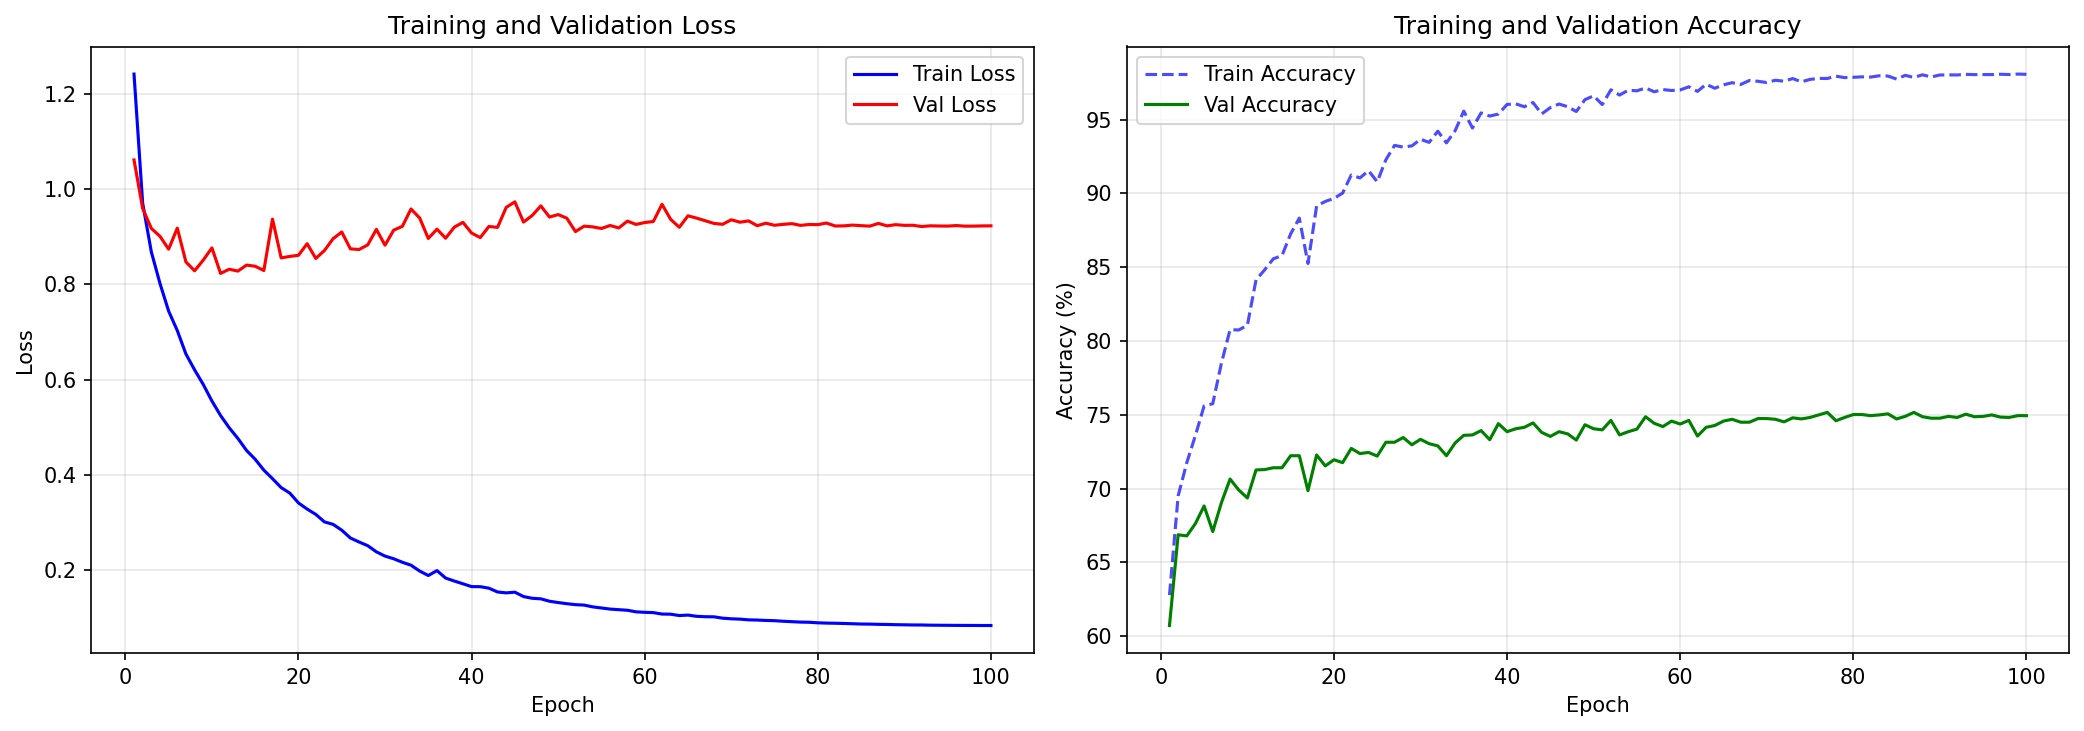
\includegraphics[width=\textwidth]{checkpoints/final/training_curves.png}
\caption{训练过程曲线：(左)训练集与验证集Loss曲线，(右)训练集与验证集Accuracy曲线}
\label{fig:training_curves}
\end{figure}

从训练曲线可以观察到：

\begin{enumerate}[leftmargin=2em]
    \item \textbf{训练Loss}持续下降，从初始的1.24降至0.08，模型在训练集上拟合良好；
    \item \textbf{验证Loss}在约25个epoch后开始上升，出现过拟合趋势。训练集准确率达到98.07\%，而验证集准确率为75.16\%，过拟合差距约23\%；
    \item \textbf{余弦学习率衰减}使学习率在训练后期缓慢下降，有利于精调模型参数；
    \item \textbf{最优模型}出现在第77个epoch，验证准确率75.16\%；
    \item 数据增强将过拟合差距从约27\%降低至约23\%，有效缓解了过拟合。
\end{enumerate}

\subsection{测试集评估}

最优模型在独立测试集上的分类准确率为\textbf{74.42\%}。各类别的分类准确率如表~\ref{tab:per_class}所示。

\begin{table}[H]
\centering
\caption{各类别测试集分类准确率}
\label{tab:per_class}
\begin{tabular}{lcc}
\toprule
\textbf{类别} & \textbf{中文名称} & \textbf{准确率} \\
\midrule
AnnualCrop & 一年生作物 & 76.08\% \\
Forest & 森林 & 93.74\% \\
HerbaceousVegetation & 草本植被 & 69.50\% \\
Highway & 高速公路 & 48.40\% \\
Industrial & 工业区 & 85.53\% \\
Pasture & 牧场 & 79.48\% \\
PermanentCrop & 多年生作物 & 60.21\% \\
Residential & 住宅区 & 76.28\% \\
River & 河流 & 65.48\% \\
SeaLake & 海洋/湖泊 & 85.65\% \\
\midrule
\textbf{平均} & & \textbf{74.42\%} \\
\bottomrule
\end{tabular}
\end{table}

从各类别准确率可以看出：

\begin{itemize}[leftmargin=2em]
    \item \textbf{高准确率类别}：Forest（93.74\%）、SeaLake（85.65\%）、Industrial（85.53\%）——这些类别具有明显的视觉特征；
    \item \textbf{低准确率类别}：Highway（48.40\%）、PermanentCrop（60.21\%）、River（65.48\%）——这些类别的视觉特征与其他类别存在较大重叠。
\end{itemize}

\subsection{混淆矩阵分析}

图~\ref{fig:confusion}展示了混淆矩阵。

\begin{figure}[H]
\centering
\begin{tabular}{c}
\toprule
\textbf{混淆矩阵} \\
\midrule
\small
\begin{tabular}{l*{10}{r}}
 & \rotatebox{70}{AnnualCrop} & \rotatebox{70}{Forest} & \rotatebox{70}{HerbVeg} & \rotatebox{70}{Highway} & \rotatebox{70}{Industrial} & \rotatebox{70}{Pasture} & \rotatebox{70}{PermCrop} & \rotatebox{70}{Residential} & \rotatebox{70}{River} & \rotatebox{70}{SeaLake} \\
\midrule
AnnualCrop & \textbf{334} & 1 & 13 & 16 & 1 & 17 & 35 & 1 & 15 & 6 \\
Forest & 0 & \textbf{419} & 2 & 1 & 0 & 12 & 0 & 0 & 1 & 12 \\
HerbVeg & 9 & 2 & \textbf{303} & 20 & 8 & 11 & 55 & 15 & 12 & 1 \\
Highway & 31 & 2 & 24 & \textbf{181} & 13 & 12 & 27 & 29 & 55 & 0 \\
Industrial & 1 & 0 & 4 & 13 & \textbf{325} & 0 & 4 & 31 & 2 & 0 \\
Pasture & 5 & 9 & 8 & 7 & 0 & \textbf{213} & 13 & 2 & 9 & 2 \\
PermCrop & 43 & 0 & 37 & 30 & 6 & 14 & \textbf{230} & 12 & 8 & 2 \\
Residential & 3 & 0 & 31 & 27 & 7 & 2 & 31 & \textbf{328} & 1 & 0 \\
River & 19 & 5 & 5 & 79 & 3 & 15 & 9 & 7 & \textbf{275} & 3 \\
SeaLake & 3 & 43 & 3 & 1 & 0 & 4 & 0 & 3 & 11 & \textbf{406} \\
\bottomrule
\end{tabular}
\end{tabular}
\caption{测试集混淆矩阵}
\label{fig:confusion}
\end{figure}

从混淆矩阵可以识别出以下主要混淆模式：

\begin{enumerate}[leftmargin=2em]
    \item \textbf{Highway $\leftrightarrow$ River}：高速公路被误分为河流的比例最高（55个Highway样本被误分为River），两者在遥感图像中均呈现为细长的线性结构；
    \item \textbf{PermanentCrop $\leftrightarrow$ AnnualCrop/HerbaceousVegetation}：多年生作物与一年生作物、草本植被在颜色和纹理上高度相似；
    \item \textbf{Forest $\leftrightarrow$ SeaLake}：部分森林图像被误分为海洋/湖泊（43个SeaLake样本被误分为Forest），可能是由于森林中的阴影区域与水体相似；
    \item \textbf{HerbaceousVegetation $\leftrightarrow$ PermanentCrop}：55个HerbaceousVegetation样本被误分为PermanentCrop。
\end{enumerate}

%============================================================
\section{权重可视化与空间模式分析}
%============================================================

\subsection{第一层权重可视化}

将训练好的第一层隐藏层权重矩阵$\mathbf{W}_1 \in \mathbb{R}^{3072 \times 1024}$的每一列恢复为32$\times$32$\times$3的RGB图像进行可视化。图~\ref{fig:weights}展示了前64个神经元的权重图像。

\begin{figure}[H]
\centering

\includegraphics[width=\textwidth]{checkpoints/final/first_layer_weights.png}
\caption{第一隐藏层权重可视化（前64个神经元）}
\label{fig:weights}
\end{figure}

\subsection{空间模式与颜色分析}

通过观察权重可视化结果，可以总结以下空间模式：

\begin{enumerate}[leftmargin=2em]
    \item \textbf{颜色偏好模式}：
    \begin{itemize}
        \item 部分神经元呈现明显的\textbf{绿色主导}，这些权重可能对森林、牧场、草本植被等绿色覆盖区域敏感；
        \item 部分神经元呈现\textbf{蓝色主导}，可能对河流、海洋/湖泊等水体区域敏感；
        \item 部分神经元呈现\textbf{灰色/棕色主导}，可能对高速公路、工业区等人工建筑区域敏感；
        \item 部分神经元呈现\textbf{红色/暖色主导}，可能对AnnualCrop、PermanentCrop等农田区域敏感。
    \end{itemize}

    \item \textbf{空间纹理模式}：
    \begin{itemize}
        \item 部分权重呈现\textbf{均匀分布}的纹理，充当全局颜色检测器，提取图像的整体色调特征；
        \item 部分权重呈现\textbf{中心-边缘对比}模式，类似于传统计算机视觉中的中心环绕滤波器，可检测局部对比度；
        \item 少数权重呈现\textbf{水平/垂直条纹}模式，可能对高速公路、河流等线性结构敏感。
    \end{itemize}

    \item \textbf{与类别的关联}：
    \begin{itemize}
        \item 绿色主导的权重与Forest、Pasture、HerbaceousVegetation类别的分类密切相关；
        \item 蓝色主导的权重对River和SeaLake的区分至关重要；
        \item 灰色/低饱和度权重更倾向于检测Highway和Industrial等人工地物。
    \end{itemize}
\end{enumerate}

值得注意的是，由于MLP将图像展平为向量，权重无法像卷积神经网络那样保留明确的空间局部性。因此，第一层权重更多表现为\textbf{全局颜色和亮度模式检测器}，而非局部纹理检测器。

%============================================================
\section{错例分析}
%============================================================

图~\ref{fig:misclassified}展示了测试集中的部分分类错误样本。

\begin{figure}[H]
\centering
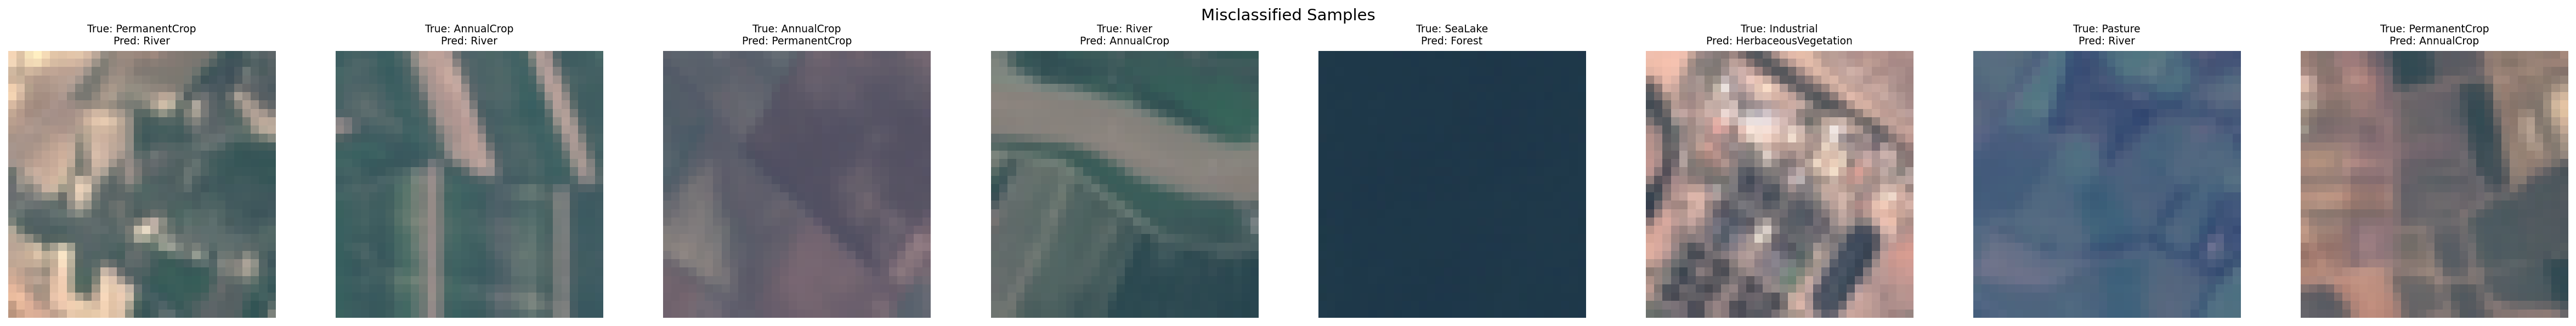
\includegraphics[width=\textwidth]{checkpoints/final/misclassified.png}
\caption{测试集分类错误样本示例}
\label{fig:misclassified}
\end{figure}

对典型错例的分析如下：

\begin{enumerate}[leftmargin=2em]
    \item \textbf{PermanentCrop $\rightarrow$ River}：部分多年生作物区域（如果园灌溉区域）可能包含水体特征，在像素级别上与河流存在相似性。MLP无法利用空间上下文信息来区分"农田中的水渠"与"自然河流"。

    \item \textbf{AnnualCrop $\rightarrow$ PermanentCrop}：一年生作物与多年生作物在遥感图像中均表现为规则排列的绿色农田，仅凭颜色和纹理特征难以区分。两者的主要区别在于种植模式和生长周期，这些时序信息无法从单张图像中获取。

    \item \textbf{SeaLake $\rightarrow$ Forest}：部分水体图像周围被茂密的森林环绕，图像中混合了深蓝色水体和深绿色植被，导致模型倾向于将其分类为森林。

    \item \textbf{Highway $\rightarrow$ River}：这是最典型的混淆类型。高速公路和河流在遥感图像中均呈现为细长的线性结构，且都可能呈现灰色或深色调。区分两者的关键特征——河流的弯曲自然形态与高速公路的直线人工形态——在展平为向量后被丢失。

    \item \textbf{Pasture $\rightarrow$ River}：部分牧场区域中可能存在小溪或水渠，使得图像中混合了绿色和蓝色特征，导致模型误判。
\end{enumerate}

\textbf{错因总结}：MLP的主要局限在于将图像展平为向量后\textbf{丢失了空间结构信息}，无法建模像素之间的局部关系和全局上下文。这导致模型难以区分视觉上相似但语义不同的地物类别。卷积神经网络（CNN）通过局部感受野和权值共享能够更好地提取空间特征，预期在此任务上会有显著更好的表现。

%============================================================
\section{代码结构说明}
%============================================================

项目代码采用模块化设计，各模块功能如表~\ref{tab:code_structure}所示。

\begin{table}[H]
\centering
\caption{代码模块结构}
\label{tab:code_structure}
\begin{tabular}{llp{8cm}}
\toprule
\textbf{模块} & \textbf{文件} & \textbf{功能} \\
\midrule
自动微分 & \texttt{autograd.py} & Tensor类，计算图构建，反向传播自动微分 \\
数据加载 & \texttt{dataloader.py} & EuroSAT数据加载、预处理、数据增强、划分、DataLoader \\
模型定义 & \texttt{model.py} & Linear层、MLP类、权重保存/加载 \\
优化器 & \texttt{optimizer.py} & SGD优化器、融合交叉熵损失、L2正则化、学习率衰减 \\
训练循环 & \texttt{train.py} & 训练流程、验证评估、最优模型保存 \\
测试评估 & \texttt{evaluate.py} & 测试准确率、混淆矩阵、错例查找 \\
超参数搜索 & \texttt{hyperparam\_search.py} & 网格搜索、随机搜索 \\
可视化 & \texttt{visualize.py} & 训练曲线、权重可视化、错例可视化 \\
主入口 & \texttt{main.py} & 命令行接口，整合所有模块 \\
\bottomrule
\end{tabular}
\end{table}

\subsection{运行方式}

\begin{lstlisting}[language=bash, caption=训练模型（使用最优默认参数）]
python3 main.py train
\end{lstlisting}

\begin{lstlisting}[language=bash, caption=自定义参数训练]
python3 main.py train --lr 0.003 --hidden-dim1 1024 \
    --hidden-dim2 256 --epochs 100 --lr-decay cosine \
    --augment --save-dir checkpoints/my_model
\end{lstlisting}

\begin{lstlisting}[language=bash, caption=超参数搜索]
python3 main.py search --search-type grid --epochs 30
python3 main.py search --search-type random --n-trials 10
\end{lstlisting}

\begin{lstlisting}[language=bash, caption=测试模型]
python3 main.py test --model-path checkpoints/final/best_model.npz
\end{lstlisting}

\subsection{环境依赖}

\begin{lstlisting}[caption=环境依赖]
Python >= 3.8
NumPy >= 1.20
Pillow >= 9.0
Matplotlib >= 3.5
\end{lstlisting}

%============================================================
\section{实验总结}
%============================================================

\subsection{主要成果}

\begin{enumerate}[leftmargin=2em]
    \item 从零实现了完整的自动微分系统，支持计算图构建和反向传播，验证了梯度计算的正确性；
    \item 实现了融合交叉熵损失函数，训练速度提升2--3倍；
    \item 在EuroSAT数据集上训练三层MLP，通过数据增强和超参数优化，最优模型测试准确率达到\textbf{74.42\%}；
    \item 通过网格搜索系统性地探索了超参数空间，发现ReLU激活函数和较小学习率对模型性能最为关键；
    \item 数据增强（翻转）是单次优化中贡献最大的措施（+4.4\%）；
    \item 第一层权重可视化揭示了模型学习到的颜色偏好和空间模式；
    \item 错例分析揭示了MLP在遥感图像分类中的核心局限——空间信息丢失。
\end{enumerate}

\subsection{改进方向}

\begin{enumerate}[leftmargin=2em]
    \item \textbf{引入卷积结构}：使用CNN替代MLP以保留空间局部性，预期可显著提升分类性能；
    \item \textbf{更多数据增强}：加入随机裁剪、颜色抖动等增强手段进一步缓解过拟合；
    \item \textbf{正则化策略}：引入Dropout和Batch Normalization进一步抑制过拟合；
    \item \textbf{更高级的优化器}：实现Adam优化器以加速收敛；
    \item \textbf{更大分辨率输入}：使用64$\times$64原始分辨率，保留更多空间细节。
\end{enumerate}

%============================================================
\section*{附录：代码与模型权重}
\addcontentsline{toc}{section}{附录：代码与模型权重}
%============================================================

\begin{itemize}[leftmargin=2em]
    \item \textbf{GitHub仓库}：\url{https://github.com/USERNAME/eurosat-mlp-classifier}
    \item \textbf{模型权重下载}：\url{https://drive.google.com/file/d/XXXXX}
\end{itemize}

\vspace{1em}
\noindent\textit{注：请将上述链接替换为实际的GitHub仓库地址和Google Drive模型权重下载地址。}

\end{document}
